\documentclass[11pt]{article}
\usepackage[a4paper,margin=25mm]{geometry}
\usepackage{amsmath,amssymb,graphicx,booktabs,tabularx,enumitem}
\usepackage[round,authoryear]{natbib}
\usepackage[colorlinks=true,allcolors=blue]{hyperref}
\usepackage{microtype}
\graphicspath{{../../reports/painter_distribution_study_v1/pdsv1-analysis-20260907/}}
\setlength{\parskip}{3pt}
\setlength{\parindent}{1em}
\setlength{\emergencystretch}{2em}
\title{Painter Names and Feature Distributions:\\Comparing Generated Images with Original Paintings}
\author{Anonymous authors\\\small Research manuscript prototype}
\date{7 September 2026}
\begin{document}
\maketitle
\begin{abstract}
An image may evoke a painter while occupying a different distribution of
measurable properties. We compare 1,006 newly generated images from Nano Banana 2,
FLUX.2 Max and a GPT Image 2 service with 70 fresh digital painting surrogates by
Monet and Cézanne. A fixed 24-brief design includes artist-free and named controls,
three repetitions and an additional generic/detailed intervention. Thirty-one
interpretable features are scaled using separate historical development works;
content weighting and processing sensitivities accompany energy discrepancy,
spread, coverage and grouped detection. In the primary comparison, the eight
named collections have generated/original variance ratios .306--.756, yet their
full-feature RBF balanced accuracies remain .893--.987. Naming reduces energy
discrepancy in all six route/painter point estimates; the four paid-route contrasts
reject the prespecified conditional randomization null after Holm correction,
whereas the OAuth naming and detail contrasts do not. Paid artist-free
variance ratios are 1.069--1.535, so concentration is not a universal property of
every generated condition. Paid-route improvements persist descriptively under
both processing sensitivities, while reference restriction and feature families
show exceptions to uniform contraction. These finite-panel findings distinguish
improved proximity from recovery of original variation. They do not establish
perceptual style equivalence; reference capture and variable service rendering
remain unresolved. All collection, measurement and numerical replay checks are
complete, with provider-reported charges of \$40.68.
\end{abstract}

\section{Introduction}
The question motivating this study is whether painter-conditioned image
generation reproduces the distribution of visual properties found across a
painter's original works. A small distance to a painter's average feature vector
does not answer this question: generated images can cluster tightly near that
average while failing to reproduce variation across works. Conversely, a
recognizable artistic reference may coexist with systematic differences in
palette, spatial organization or digital texture.

We distinguish four properties: distribution discrepancy, within-set spread,
reference coverage and painter specificity. None is an aesthetic quality score.
The measured objects are digital reproductions of paintings and generated image
files. Their comparison combines artistic choices with content, reproduction,
resizing, encoding and service behavior. Treating every detectable difference as
a failure of painter-style reproduction would overstate what the measurements identify.

The completed analysis suggests a useful, narrower hypothesis: under the tested
prompt libraries and image processing, painter-conditioned generations occupy
more concentrated and distinguishable feature distributions than the recorded
original-painting surrogates. The controlled study tests whether this pattern persists under stronger content
controls and across additional model families. Its central finding is that painter
naming can improve proximity while contracting measured spread; artist-free
controls show why these properties should not be conflated.

\section{Related work and the distinct research question}
Quantitative art research has characterized painting collections using color,
image statistics and information-theoretic measures
\citep{kim2014,lee2020,sigaki2018}. Kim et al.'s 2026 study concerns contextual
multimodal navigation through art-historical development \citep{kim2026}. Our
sampling unit and target differ: we compare within-painter distributions across
distinct works with newly generated text-to-image collections, with painter-name
and prompt-content interventions. We do not claim to replicate its art-evolution
analysis or its complete measurement system. Our fixed 31-feature representation
is the existing implementation in this project.

Asperti's recent preprint reports separation of human and generated paintings
in CLIP space and investigates preprocessing robustness, interpretable multiscale
structure and inversion \citep{asperti2026}. Thus, scatter separation alone is not
sufficient novelty for this work. We emphasize painter-conditional comparisons,
explicit artist-free controls and the effects of prompt content on a fixed
interpretable representation. We have not run CLIP or reproduced that preprint's
inversion experiments. More generally, feature-space distinctions need not have
the perceptual significance assumed by a style evaluator.

Generative-model evaluation separates fidelity and coverage for related reasons
\citep{naeem2020}. Resizing and compression can change measured differences
\citep{parmar2022}; digital-surrogate provenance is consequently part of the
experimental design rather than a minor file-handling detail. Energy statistics
provide a distributional comparison based on pairwise distances
\citep{szekely2013}, without reducing each collection to its centroid.

\section{Development evidence and design motivation}
The development analysis compares 649 digital painting surrogates (297 Monet,
106 Sisley, 141 Pissarro and 105 Cézanne) with 1,920 generated images. Its grid
crosses two requested GPT Image service aliases, three prompt methods, 16 scene
templates and four repetitions, with named and artist-free conditions. Two later,
explicitly authorized exact-payload retries complete the descriptive grid after
its original two refusals: 1,920 images from 1,922 requests. Their later timing
does not restore the original complete-grid primary. These development findings
are descriptive; they have no retrospective replacement-based inference.
The requested aliases do not attest distinct underlying model snapshots.

Named cells have generated/original sample-variance ratios .206--.376 and
scene/work-disjoint RBF balanced accuracy .940--.983. Artist-free cells also
separate strongly (.915--.990), with larger spread ratios (.369--.750).
Reweighting coarse title/prompt-derived content classes changes the variance
ranges to .211--.372 and .378--.728, respectively. Matched-size disjoint original
splits have much smaller median energy discrepancies (.1635--.2149) than
named/original comparisons (1.6776--2.1419). These repeated splits describe one
finite corpus, not independent studies or a calibrated equivalence margin.

Earlier family-specific distance comparisons favor by-name prompting in 19 of
24 combinations of alias, painter and feature family; style-plus-aspects is closest
in five. Explicit
style instructions increase distance relative to by-name prompting in all 24;
adding aspects has mixed directions. Cross-alias RBF transfer remains strong
(median balanced accuracy .965), consistent with shared generated-image or
capture signatures. Together, these observations motivate model-family breadth,
better content labels and a focused prompt intervention. They do not establish
best achievable prompting or isolate a painter-style mechanism. The completed
historical report retains every numeric result, projection and split membership;
its different reference corpus is not pooled with the new study.

\section{Controlled study design}
\subsection{Choice of expansion axis}
We expand model-family breadth and improve the comparison target before adding
more painters. New collection focuses on Monet and Cézanne. The existing four
painter results are retained as development evidence. This is a disclosed
two-painter case study, chosen after earlier outcomes were known; it cannot
estimate the prevalence of the phenomenon across all painters or traditions.

The research grid uses the same 24 content briefs across both painters, with three
repetitions, named and artist-free conditions on three routes, plus a generic
named condition on OAuth: 1,008 research slots. Eighteen separate technical
requests and at most 24 bounded transient-error retries give a ceiling of 1,050
attempts, including at most 612 paid attempts. The spending ceiling is \$75,
including the pilot and retries. Successful images are never regenerated or
selected among alternatives. Sample counts reflect affordability and design
coverage; they do not establish power for an image-space effect.

The reference target initially specified 48 fresh works per painter and 12
content strata. The recorded identity audit selects 64 Monet and 48 Cézanne
candidates outside the prior exposure indexes. Original delivery encounters
Wikimedia rate limits; a separately frozen successor follows its supported
thumbnail policy. Nonupsampled standard delivery supports 38 Monet and 33
Cézanne candidates. All 71 deliveries succeed. Single-maintainer LLM visual
coding excludes one figure-led Cézanne, leaving 38 Monet and 32 Cézanne works.
These unequal counts are disclosed before measurement; no 48-work panel or
fully balanced 12-stratum design is claimed.

Visually coded water, built and land organization replaces geographic-name
heuristics. Counts are 21/4/13 for Monet and 3/11/18 for Cézanne. The primary
comparison gives original works equal weight and generated images the same fixed
class masses as their target reference. Eight shared briefs per class support this
weighting. Collected-mixture and equal-class sensitivities are also required;
the latter heavily weights Cézanne's three water scenes. Mixed annotations remain
flagged, with an exclusion sensitivity. This is coarse content control, not exact
scene matching or independent expert annotation. Independent photographic
capture pairs have not been established. Thumbnail and alternate-file provenance
cannot substitute for evidence of distinct capture events.

\subsection{Technical pilot results}
All six requests per route return decodable images. Google
\texttt{gemini-3.1-flash-image} through the pinned Google AI Studio provider
returns 1024-square JPEGs, costing \$0.4105 in total. BFL \texttt{flux.2-max}
through its pinned provider returns 1024-square PNGs, costing \$0.4200.
The local OAuth \texttt{gpt-image-2} comparator returns nonsquare PNGs with
short sides 1121--1126 and reports low rather than requested medium quality.
No paid fallback, retry, prompt rewrite or feature-based pilot selection occurs.

The completed research collection retains 1,006 images from 1,008 fixed slots:
288 Nano Banana 2, 288 FLUX.2 Max and 430 OAuth outputs. Two OAuth generic-named
Cézanne slots receive moderation refusals and remain missing. One complete FLUX
502 receives one successful exact-payload technical retry under the frozen rule.
Including 18 pilot attempts and this retry, there are 1,027 physical attempts,
589 paid. Provider-reported charges total \$40.6819185. The failed FLUX call omits
cost; its raw null remains, with a full \$5 contingency, giving conservative
accounting \$45.6819185 against the \$75 ceiling. No unresolved outcome or
unclassified cost remains. OpenRouter's published failed-image billing waiver
\citep{openrouter2026imageapi} is not substituted for an individual receipt.

All paid research outputs are 1024-square: Google JPEG and BFL PNG. OAuth returns
430 PNGs with short sides 1087--1254 pixels; eight are square. Of these, 424 report
low quality and six report medium despite all requesting medium. The six medium
outputs are artist-free (three per painter); all named outputs report low.
These response fields do not attest an immutable model or comparable rendering.
OAuth is therefore a separate service comparison. A prompt contrast on that route
includes any prompt-induced service handling; it cannot isolate painter naming
at fixed delivered quality. No output is filtered by its reported quality.
Symmetric 256-pixel and common-JPEG sensitivities probe processing effects but
cannot undo earlier encoding or generation-quality differences.

\section{Distribution measurements and statistical analysis}
\subsection{Feature representation and processing}
Each image is represented by 11 color, eight spatial and 12 digital-texture
features. Color includes lightness and chroma location/spread, hue organization,
and multiscale chromatic differences. Spatial features include spectral shape,
orientation organization, gradients and quadrant differences. Texture includes
wavelet energies and trends, local binary-pattern entropies and local luminance
variation. These are measurements of digital images, not direct measurements of
physical brushstroke relief or a validated complete definition of painter style.

The primary normalization applies EXIF orientation, converts valid embedded
profiles to sRGB, assumes sRGB when compatible unprofiled data are present,
rejects nonopaque images and preserves aspect ratio at a 512-pixel short side.
It uses Lanczos resampling without upsampling or discretionary cropping.
Each coordinate is centered by the development median and divided by the
development interquartile range. Development painters receive equal total mass;
no generated or new reference feature is used to fit that scaler.


\subsection{Distribution discrepancy and spread}
Let $x_i$ and $y_j$ be standardized reference and generated vectors, with
nonnegative weights $a_i$ and $b_j$ that each sum to one. We report the empirical
V-statistic energy discrepancy
\begin{align}
\widehat{\mathcal E}(X,Y)={}&2\sum_{i,j}a_i b_j\lVert x_i-y_j\rVert_2
-\sum_{i,k}a_i a_k\lVert x_i-x_k\rVert_2\nonumber\\
&-\sum_{j,l}b_j b_l\lVert y_j-y_l\rVert_2.
\label{eq:energy}
\end{align}
All pairwise terms contribute; the reference mean is not the sole comparison
target. The finite-sample V-statistic has a nonzero sampling baseline even when
independent samples come from one common population.

We report the ratio of total within-group sample variances for ordinary
unweighted data. Weighted analyses use the population-form trace
$\sum_i a_i\lVert x_i-\sum_k a_k x_k\rVert^2$ in both numerator and denominator.
The sample and population definitions have different finite-sample denominators.
A complementary robust summary divides the sum of squared generated coordinate
IQRs by the corresponding reference sum. Undefined coordinate ratios remain
undefined rather than being stabilized by an arbitrary constant.


\subsection{Content control and sensitivity analyses}
The controlled reference panel has now produced all 210 expected feature vectors
under three processing pipelines, without measurement failures or duplicate raw
image hashes. Recomputing those vectors from retained source bytes reproduces
all records. Both sensitivity scalers were fitted first, from 442 remeasurements
of the same 221 historical development works. All 1,006 selected generated images produce their 3,018 expected vectors without
measurement failures or duplicate raw hashes. Generated features are first
accessed after terminal collection, and retained raw bytes support exact replay.

For painter $p$, let $N_{pc}$ denote the number of reference works in content
class $c$, $N_p$ the total, and $n_{pc}$ the number of available generated
observations in a particular route/condition cell. The primary weights are
\begin{equation}
 a_i=1/N_p,\qquad b_j=\frac{N_{pc}}{N_p n_{pc}}\quad\text{for }j\in c.
\end{equation}
Each cell is assigned 72 slots: eight briefs per content class, each repeated
three times. Missing outputs redistribute only their own class's fixed mass;
a required class with no measured output makes that comparison unavailable.
The weighting is conditional on intended generated content, whose adherence has
not been independently judged. Images are not discarded for failing to resemble
a painter or for depicting the intended scene imperfectly. Effective weight size
$1/\sum_j b_j^2$ is reported separately from the number of image files.

Primary energy discrepancy and the two spread ratios use all 31 standardized
features. Color, spatial and texture subsets remain descriptive. Prespecified
sensitivities use the collected generated mixture, one-third mass per content
class, only unambiguous reference annotations, only retained reference files with native
short sides at least 1024 pixels, and initial-attempt successes alone. The
annotation and native-size restrictions redefine their reference class masses
from the retained subset and are labeled accordingly. A 256-pixel short side
and common JPEG encoding at quality 90 with 4:2:0 subsampling additionally probe
processing sensitivity. No histogram, palette or texture matching is performed.

For the new disjoint original/original baseline, each of 999 deterministic draws
selects two nonoverlapping sets of $\lfloor N_{pc}/2\rfloor$ works per class and a
generated set with the same class counts, without replacement. All sets retain
the declared class masses. The resulting group sizes are 18 for Monet and 15 for
Cézanne; the latter includes only one water work per group. The repeated draws
characterize this finite panel and do not create independent reference samples.

Secondary coverage uses an original-centered ball with radius $r_i$ equal to
the distance to the third nearest distinct reference work:
\begin{equation}
 \widehat{C}=\sum_i a_i\,\mathbf{1}
 \!\left\{\min_j\lVert x_i-y_j\rVert_2\leq r_i\right\}.
\end{equation}
We report all-available coverage and 100 uniform generated subsamples of size
$\min(N_p,n_p)$, without replacement. These neighborhood measurements depend on
sample size and representation and are not artistic-completeness scores.

Fixed linear/RBF kernel-ridge detection uses six whole-brief folds and disjoint
reference works, with no tuning or PCA input. Reference folds are assigned by
content-stratified identity hashes, so sparse classes are distributed across
folds. Training assigns equal total mass to original and generated labels and
matches content masses within each label; held-out balanced accuracy and AUC use
the same target masses. Eight folds over assigned collection batches provide a
timing sensitivity; the batches do not identify independent service sessions.
Every split and prediction is retained. For visualization, each painter has one
common PCA fit with half the mass on originals and half shared equally across
seven generated cells, using the primary content weights. Original-only PCA is
also retained. Every point is shown under shared within-painter axes. Painter
specificity compares each named cell with both reference painters under the
same one-third-per-class mixture, separately from its absolute discrepancy.

\subsection{Assignment, execution and missingness}
The reference, prompt inventory, endpoints, scaling and analysis are committed
before evaluation features are extracted. Repetitions are assigned to eight
batches with originally planned offsets 0, 3, 6, 9, 24, 27, 30 and 33 hours.
Within-route condition order is randomized, with at most one active call per
route and globally staggered starts at least five seconds apart. All attempts,
refusals, technical retries and actual timestamps are preserved.

Three interrupted collection components remain permanently closed: a generic
HTTP 400 guard stopped on a moderation refusal; a later complete FLUX 502 stopped
on missing cost; and the waiting recovery closed when the user requested immediate
completion. Each correction has disjoint, predecessor-bound evidence and precedes
all generated-feature measurement. The final 504 untouched slots run consecutively
in batches 4--7 on 7 September, 00:29:19--02:01:37 UTC, under unchanged scientific
assignments and rate limits. The complete 33-hour schedule was not executed.
The final finite-slot view retains both refusals and the sole technical retry;
it does not silently replace a slot or claim independent backend sessions.

Prospective synthetic qualification passes for the eight paired all-31 prompt
contrasts: six named-versus-free and two detailed-versus-generic OAuth contrasts.
Two fixed-seed phases each use 10,000 trials in 24 null cells covering pair counts,
contribution heterogeneity, window drift and endpoint dependence. Actual tests use
99,999 Monte Carlo sign draws and Holm adjustment. Their sharp null concerns
availability and features under the randomized slot policy, conditional on the
finite reference, with no interference. Service carryover and retry-induced timing
remain limitations. This qualification does not validate absolute-distribution
p-values, oeuvre-sampling intervals or actual image-space power. Absolute gaps and
leave-batch/brief ranges remain descriptive. Ordinary image-level bootstrap
intervals are not justified by the number of files alone.
No significance-based sampling extension, silent replacement of missing outputs
or retrospective change to a sealed endpoint is allowed. Human construct validation remains unperformed. Absolute discrepancy and spread
are descriptive; only the eight prespecified prompt contrasts carry conditional
randomization p-values.

\subsection{Paired statistic and conditional interpretation}
For a matched before/after pair $(A_i,B_i)$ with fixed class-adjusted weight
$b_i$, define $C(v)=\sum_j a_j\lVert v-x_j\rVert_2$ and
$T(v)=\sum_i b_i(\lVert v-A_i\rVert_2+\lVert v-B_i\rVert_2)$. The contribution
\begin{equation}
 c_i=b_i\{2[C(B_i)-C(A_i)]-[T(B_i)-T(A_i)]\}
\end{equation}
satisfies $\sum_i c_i=\widehat{\mathcal E}(X,B)-\widehat{\mathcal E}(X,A)$.
Thus the contrast retains the within-generated pairwise terms; it is not a
contrast of mean-to-centroid distances. Complementary condition swaps produce
$\sum_i s_i c_i$ for assignment signs $s_i\in\{-1,1\}$. For the three-condition
OAuth groups, each pairwise comparison conditions on the third condition's
position in the uniformly randomized order.

A contrast uses complete measured pairs sharing a brief, repetition and assigned
batch. If fewer than 24 pairs or 12 distinct briefs survive, or a required
content class is absent, its endpoint is unavailable and retains $p=1$ in the
fixed eight-test family. This is distinct from the all-available descriptive
comparison. Two-sided Monte Carlo p-values use $(1+e)/(1+99999)$, where $e$ counts
sign-draw statistics at least as extreme in absolute value, including numerical
ties. Leave-one-batch and leave-one-brief estimates assess sensitivity without
being labeled confidence intervals. The sharp assignment null covers both
availability and measured features for the full fixed slot policy, including its
bounded technical retry rule; it is stronger than equality of expected distances.
Treatment-dependent service duration and retry delays can affect later calls,
so the randomization calculation does not remove the no-interference limitation.

\section{Controlled results}
\subsection{Proximity and spread are distinct}
All 14 primary cells and all eight inferential endpoints are available.
Table~\ref{tab:primary} compares the full distributions, not just painter means.
Every named condition has less total empirical variance than its reference
(ratios .306--.756). Detailed named ratios are .354--.756; the two generic-named
OAuth cells are .306 and .395. Naming also contracts spread relative to the
corresponding artist-free condition in all six route/painter comparisons.
However, paid artist-free ratios are 1.069--1.535. The data therefore support
concentration of these painter-conditioned collections, not an intrinsic claim
that generated images always have less variation.

\begin{table}[ht]
\centering\small
\begin{tabular}{lllrrrr}
\toprule
Painter & Route & Prompt & Energy & Variance & IQR sum & RBF BA\\
\midrule
Monet & NB2 & Free & 4.188 & 1.086 & 1.131 & 0.939\\
 & NB2 & Named & 3.342 & 0.756 & 0.966 & 0.906\\
 & FLUX & Free & 1.990 & 1.071 & 0.941 & 0.901\\
 & FLUX & Named & 1.365 & 0.354 & 0.377 & 0.953\\
 & OAuth & Free & 2.567 & 0.863 & 1.176 & 0.960\\
 & OAuth & Named & 2.333 & 0.478 & 0.586 & 0.962\\
 & OAuth & Generic & 2.370 & 0.306 & 0.330 & 0.987\\
\midrule
Cézanne & NB2 & Free & 4.704 & 1.535 & 1.371 & 0.970\\
 & NB2 & Named & 2.886 & 0.716 & 0.785 & 0.977\\
 & FLUX & Free & 1.700 & 1.069 & 0.950 & 0.903\\
 & FLUX & Named & 0.804 & 0.492 & 0.567 & 0.893\\
 & OAuth & Free & 1.941 & 0.787 & 0.928 & 0.958\\
 & OAuth & Named & 1.884 & 0.512 & 0.461 & 0.920\\
 & OAuth & Generic & 2.166 & 0.395 & 0.299 & 0.918\\
\bottomrule
\end{tabular}
\caption{Primary 512-pixel, all-31, reference-content-weighted results.
Variance and squared-IQR-sum values are generated/original ratios.
BA holds out whole briefs and distinct original works. Each cell has 72 images
except Cézanne/OAuth/generic (70); references have 38 Monet and 32 Cézanne works.
NB2 denotes Nano Banana 2; FLUX denotes FLUX.2 Max; OAuth is the GPT Image 2
service. Named uses detailed briefs; Generic uses generic named briefs.}
\label{tab:primary}
\end{table}

The contraction is uneven across feature families. Among the eight named cells,
color variance ratios range .291--.745 and digital texture .143--.460. Spatial
ratios range .665--1.520, with four detailed named cells above one. Thus, lower
aggregate spread does not mean lower variation in every type of visual property.
These family results are descriptive and do not identify a physical brushstroke
or perceptual-diversity mechanism.

\begin{figure}[p]
\centering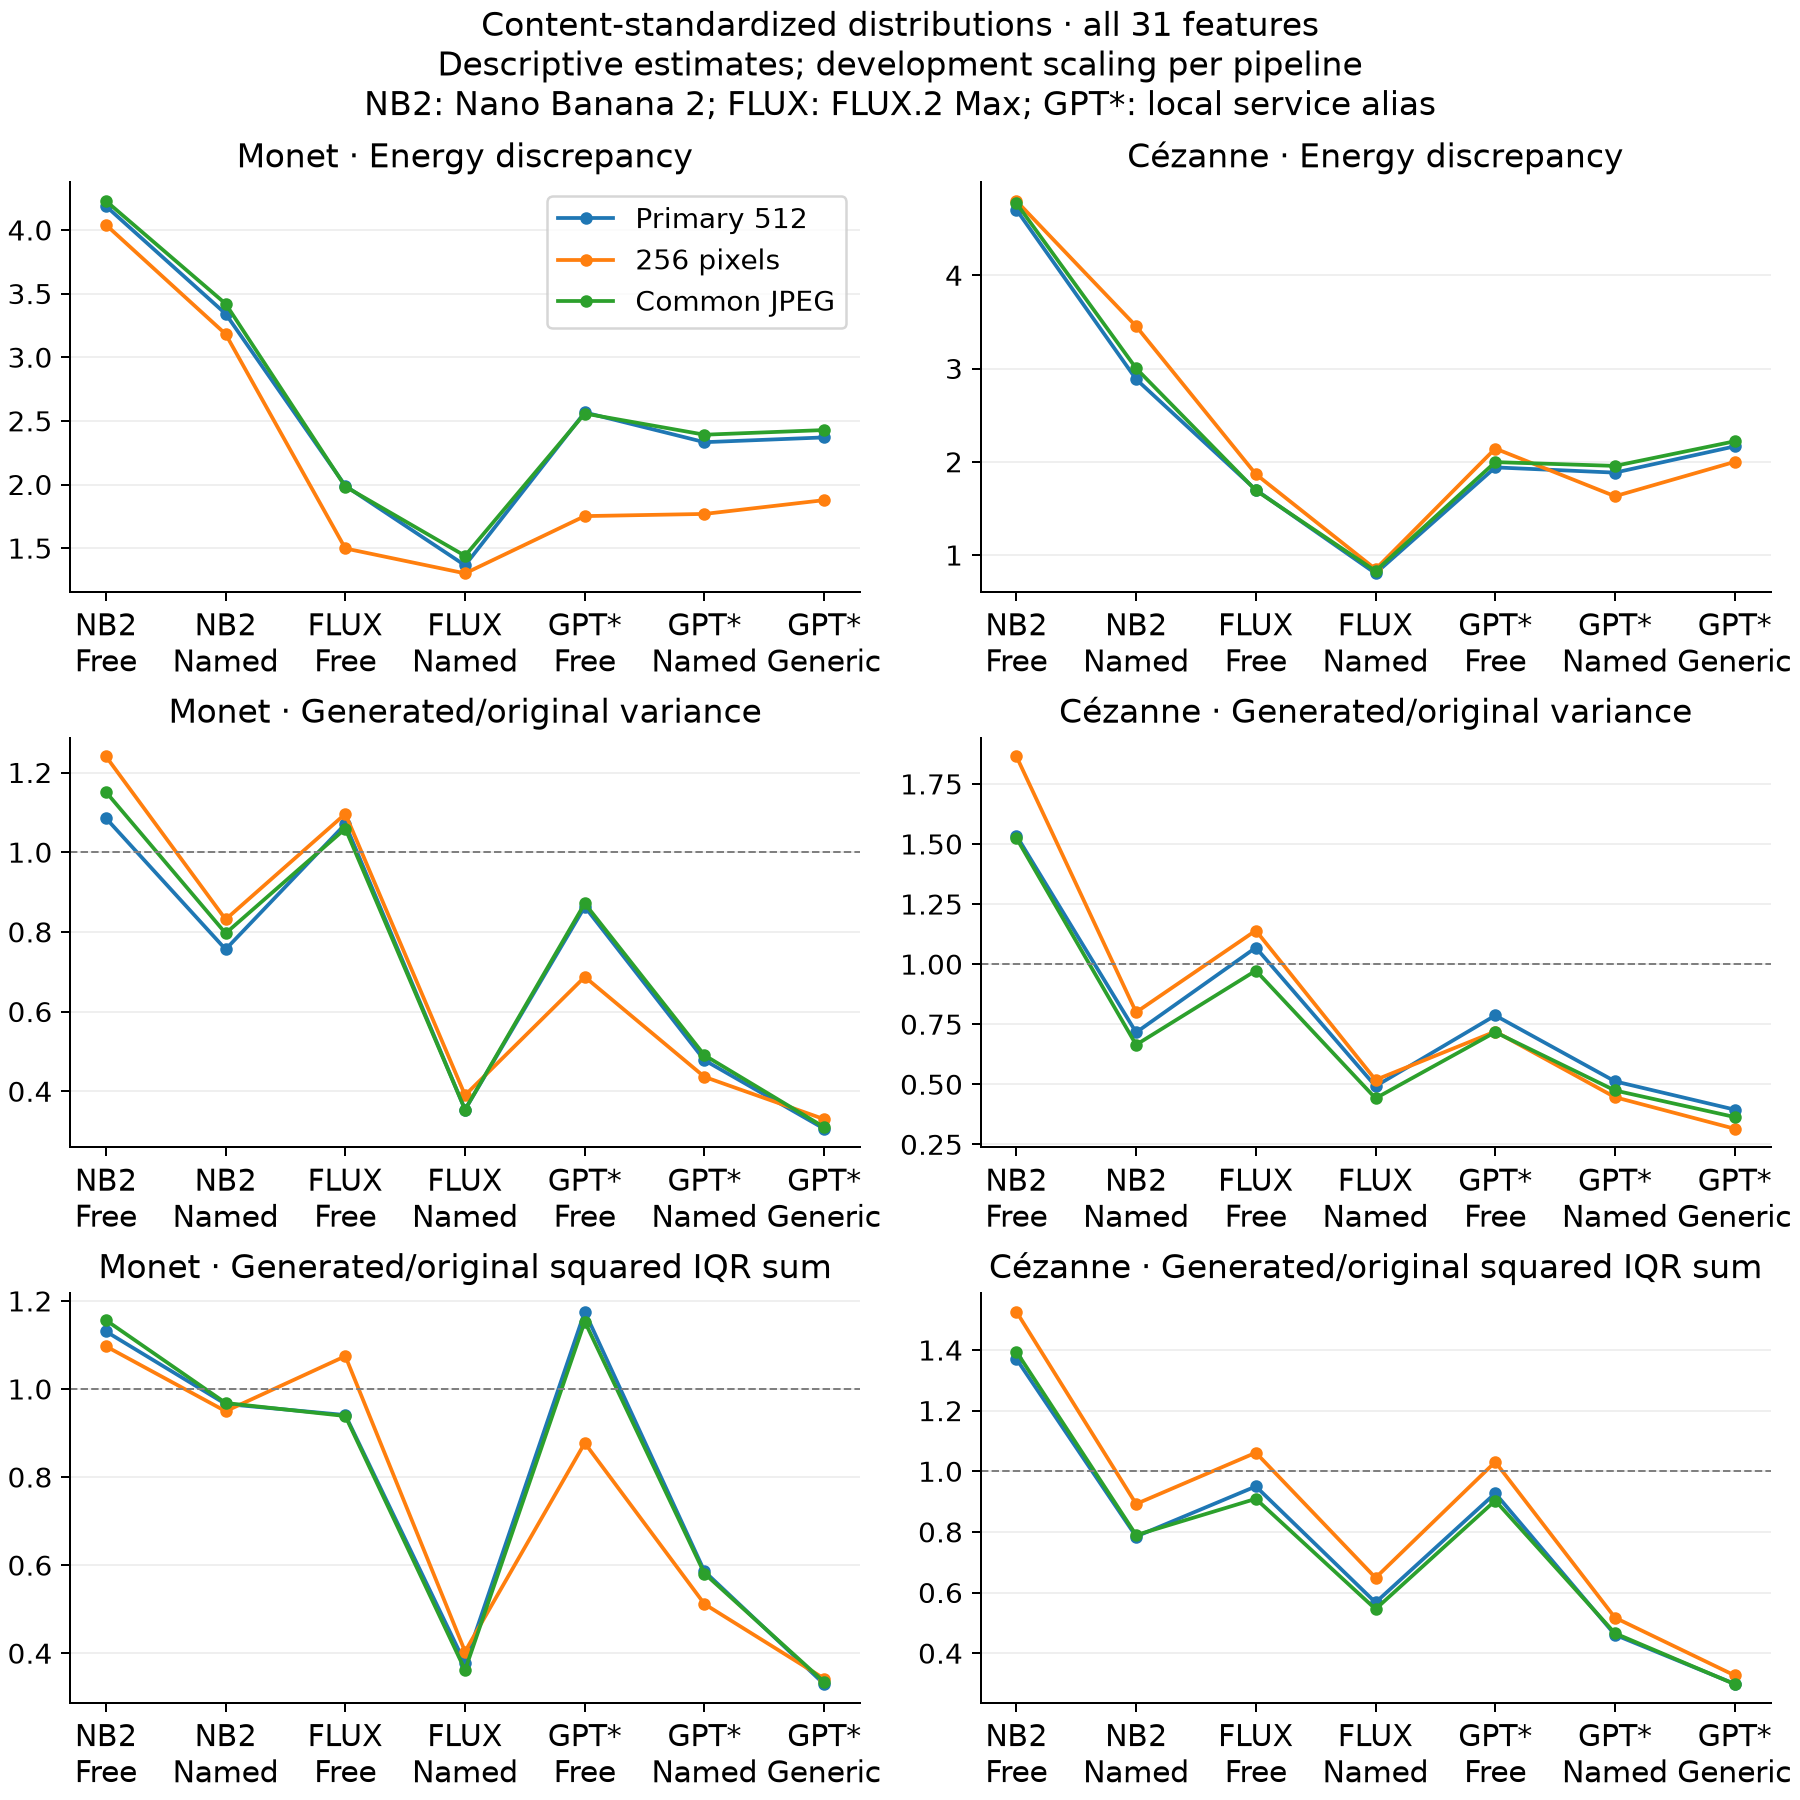
\includegraphics[width=\linewidth]{distribution_metrics.png}
\caption{Full-distribution discrepancy and two spread summaries across the three
fixed processing pipelines. Named means detailed named; Generic means generic
named. Every pipeline uses its own development-only scaler. Dashed lines mark a
spread ratio of one, not a calibrated equivalence boundary.}
\label{fig:metrics}
\end{figure}

\subsection{Scatter overlap coexists with full-space detectability}
The balanced joint PCA retains 48.4\% of weighted variation in its first two
components for Monet and 46.0\% for Cézanne. The clouds overlap in these views
(Figure~\ref{fig:controlled-pca}), with route- and condition-specific shifts and
concentration. Original-only PCA, retained in the report, explains 55.6\% and
52.2\% in two dimensions and also shows overlap. Neither projection supports a
claim of perfectly disjoint distributions.

In all 31 features, whole-brief/work-disjoint RBF balanced accuracy is .893--.987
across all 14 cells, including artist-free controls. Linear accuracy is .837--.969.
Holding out assigned batches gives .889--.987 (RBF) and .822--.969 (linear).
These fixed-model descriptive scores establish practical detectability within
the recorded evaluation splits. They do not identify which differences represent
painter style, nor provide an absolute distribution-equality test.

\begin{figure}[p]
\centering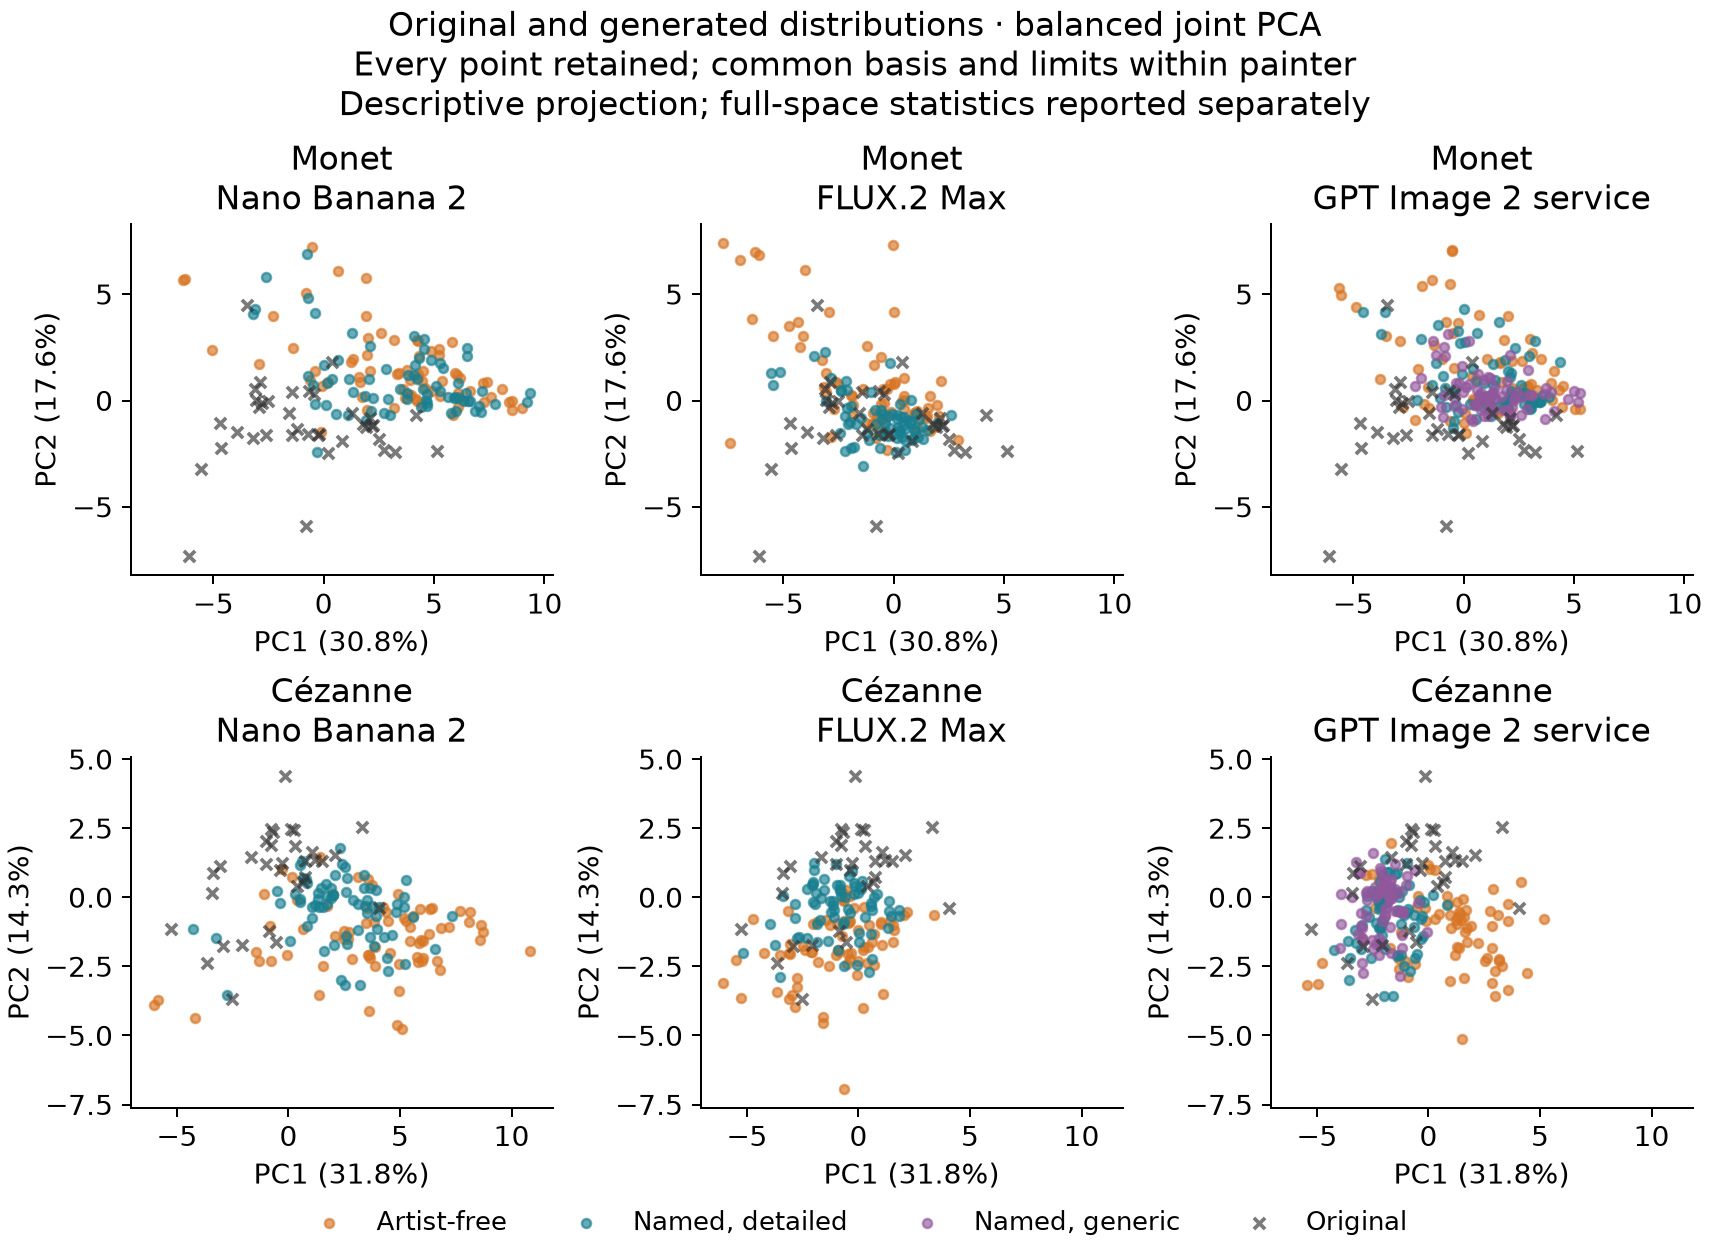
\includegraphics[width=\linewidth]{pca_balanced_joint.png}
\caption{Common painter-specific PCA with every original and generated point
retained. Each painter uses one basis and shared limits across routes. Originals
receive half the fit weight; generated cells share the other half. Overlap in
two projected dimensions coexists with strong held-out full-space detection.}
\label{fig:controlled-pca}
\end{figure}

\subsection{Painter naming improves proximity on the paid routes}
All six primary named-minus-free energy point estimates are negative
(Table~\ref{tab:contrasts}). The four paid-route contrasts reject the fixed
conditional sharp null after Holm adjustment over eight tests. Their improvements
range from .625 to 1.818 energy units. Every leave-one-brief and leave-one-batch
estimate for those four contrasts remains negative. These ranges describe the
finite design; they are not confidence intervals.

Neither OAuth naming contrast rejects after adjustment (Holm $p=.19308$ for Monet
and $p=1$ for Cézanne). The generic-to-detailed OAuth contrast is small for Monet
($-.0375$, Holm $p=1$) and larger for Cézanne ($-.2723$, Holm $p=.0928$), using
70 complete Cézanne pairs because both refusals occur in its generic condition.
Non-rejection does not establish no effect. Detailed named OAuth images have
more empirical spread than generic ones for both painters, but this comparison
changes content specificity as well as wording; it is not a pure length effect.

\begin{table}[ht]
\centering\small
\begin{tabular}{lllrrrr}
\toprule
Route & Painter & Contrast & Pairs & Energy change & Raw $p$ & Holm $p$\\
\midrule
NB2 & Monet & Name & 72 & -0.8462 & 0.00062 & 0.0031\\
NB2 & Cézanne & Name & 72 & -1.8176 & $10^{-5}$ & $8\times10^{-5}$\\
FLUX & Monet & Name & 72 & -0.6246 & $10^{-5}$ & $8\times10^{-5}$\\
FLUX & Cézanne & Name & 72 & -0.8956 & $10^{-5}$ & $8\times10^{-5}$\\
OAuth & Monet & Name & 72 & -0.2339 & 0.06436 & 0.19308\\
OAuth & Cézanne & Name & 72 & -0.0561 & 0.61624 & 1\\
OAuth & Monet & Detail & 72 & -0.0375 & 0.773 & 1\\
OAuth & Cézanne & Detail & 70 & -0.2723 & 0.0232 & 0.0928\\
\bottomrule
\end{tabular}
\caption{Prespecified two-sided paired tests, 99,999 Monte Carlo sign draws,
Holm family size eight. Name compares artist-free with detailed named; Detail
compares generic named with detailed named. Negative values mean closer after
the intervention, on complete matched pairs. The sharp null includes availability
and features under the fixed slot/retry policy and assumes no interference.}
\label{tab:contrasts}
\end{table}

\begin{figure}[p]
\centering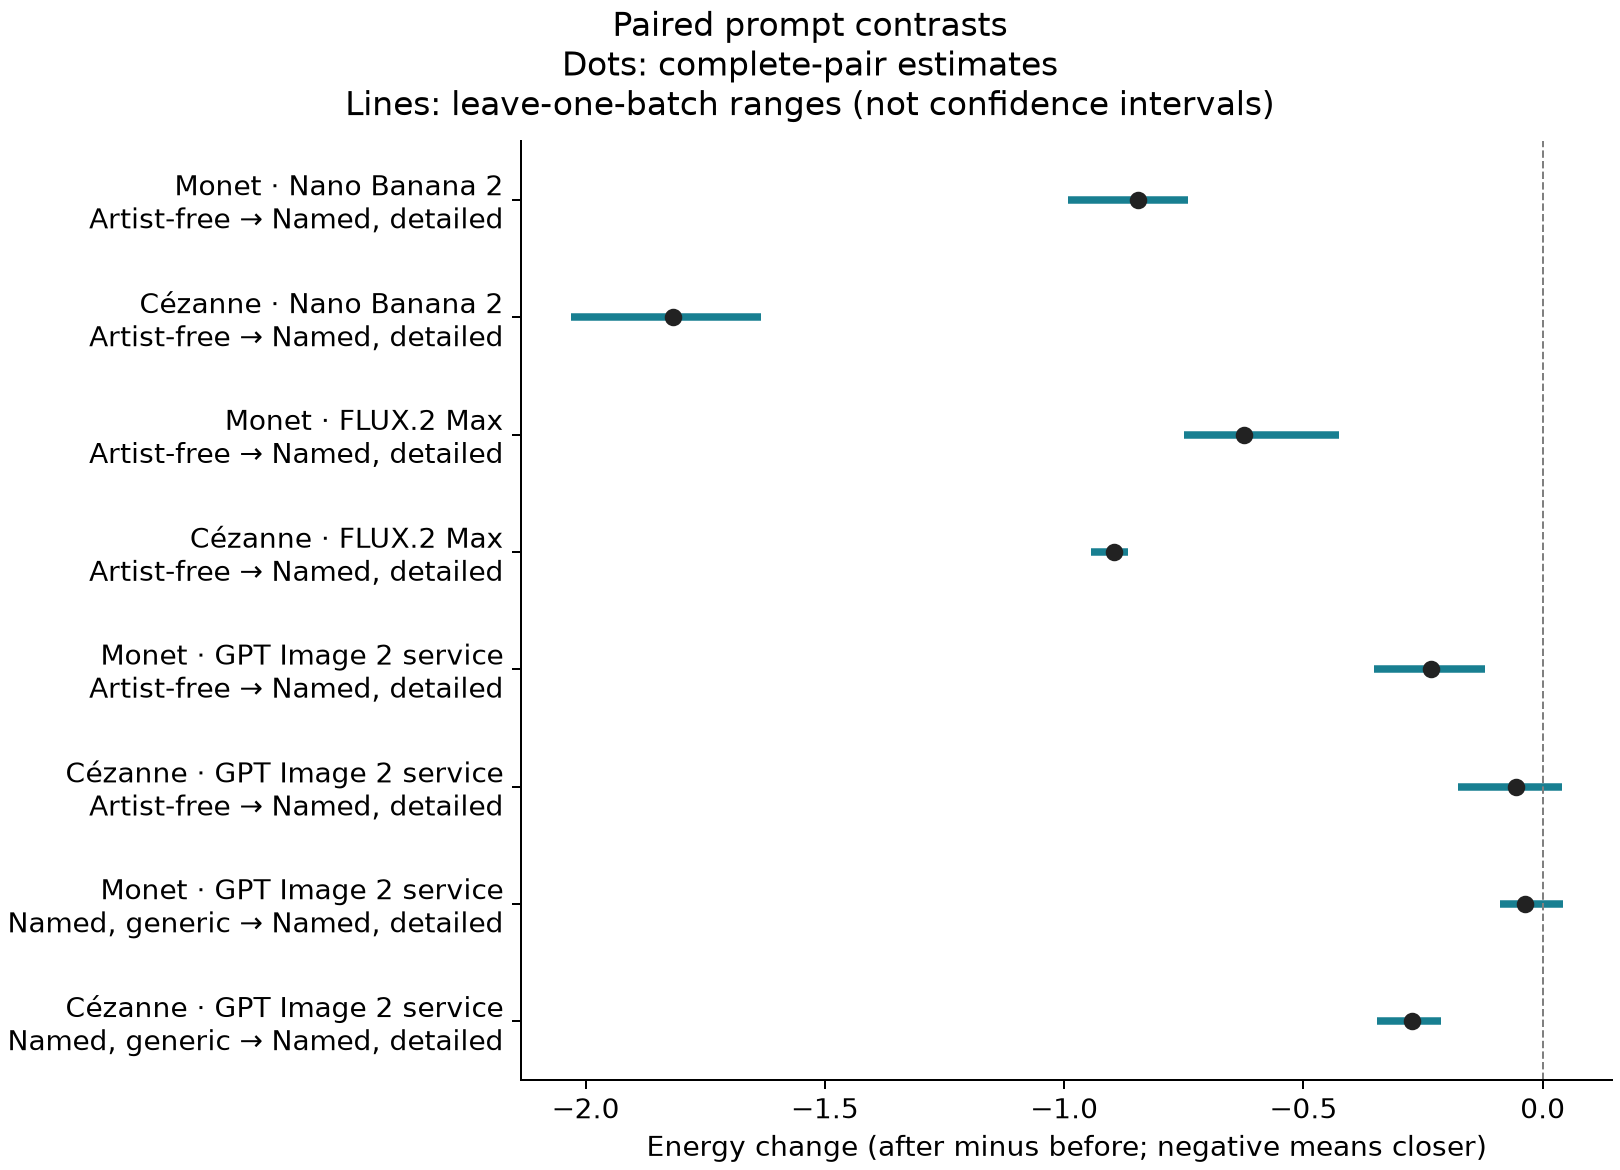
\includegraphics[width=\linewidth]{prompt_contrasts.png}
\caption{Complete-pair estimates and leave-one-assigned-batch ranges. Shared
service state and timing dependence remain limitations of the conditional tests;
the displayed lines are not uncertainty intervals for a painter's oeuvre.}
\label{fig:contrasts}
\end{figure}

\subsection{Finite-reference baselines, coverage and specificity}
Across the 14 matched-sample comparisons, original/original energy medians range
.697--.753, while original/generated medians range 1.170--5.232. Every generated
comparison has a larger median than its corresponding original split. The lowest
generated median is Cézanne/FLUX/named (1.170 versus .718); its subsample ranges
overlap the original baseline. These finite-panel draws do not establish a
population rejection or an equivalence threshold.

FLUX named outputs have the lowest primary energy among the tested routes for
both painters (1.365 Monet, .804 Cézanne), together with the highest named
all-available neighborhood coverage (.789 and .750). Equal-size subsample
coverage medians are lower (.737 and .672). For Monet/FLUX, naming improves
energy from 1.990 to 1.365 and coverage from .553 to .789, while variance contracts
from 1.071 to .354. Proximity, spread and neighborhood coverage can therefore move
in different ways; a single distance cannot describe all three.

Under equal content-class masses, five of six detailed named cells are closer to
their own reference painter than to the other painter. Nano Banana 2's Monet
condition is the exception: energy 3.687 to Monet versus 3.488 to Cézanne.
Improved proximity to a requested target thus does not guarantee painter
specificity. This two-painter comparison is descriptive and is not a validated
recognition task or a general model leaderboard.

\subsection{Processing and reference sensitivities}
For the eight named cells, total-variance ratios remain below one under both
fixed processing sensitivities: .315--.831 at 256 pixels and .310--.797 after
common JPEG encoding. All four paid-route naming effects retain their negative
descriptive energy direction under both. OAuth is less stable: Monet's naming
difference changes from $-.234$ in the primary pipeline to $+.017$ at 256 pixels.
No additional significance family is introduced for these sensitivities.

Collected-mixture, equal-content and unambiguous-reference analyses retain
aggregate variance ratios below one for all eight named cells. Some IQR-based
ratios exceed one after reweighting or reference restriction. The native-1024
restriction is particularly limited: only four Monet and 19 Cézanne reference
files remain. Nano Banana 2's Monet variance ratio becomes 1.107 in that primary
subset (1.123 at 256 pixels; 1.178 after JPEG). This is a material exception to
uniform robustness and a change in the finite comparison target. It cannot serve
as a strong independent capture control. Initial-only analysis preserves all
named cells; its only additional exclusion is the retried FLUX artist-free slot.

\section{Discussion}
The controlled results support the narrow hypothesis that these painter-named
collections differ from the recorded original-painting distributions and occupy
less aggregate feature variation. They also revise an overly broad version of
that hypothesis: the paid artist-free controls can be more dispersed than the
originals, spatial features need not contract, and a small reference restriction
reverses one aggregate result. The evidence is about the tested conditional
collections and finite digital reference panels.

The strongest prompt finding is improved proximity with contracted spread on
both paid routes. This is consistent with painter naming selecting a narrower
region of the model's output distribution, but the experiment does not identify
that internal mechanism. Better energy fit can coexist with higher coverage,
strong detection and incomplete painter specificity. Calling all of these outcomes
``style fidelity'' would conceal useful distinctions.

The next research priority is construct and reference validation, rather than
another large generation sweep. Blinded human judgments of painter recognizability
and within-set variation could test whether the interpretable measurements track
perceived style. Independent content annotation and larger, capture-documented
reference panels would address the weakest controls. Learned features can later
provide a complementary representation, with their own processing checks and
human calibration. More generated files alone would not resolve these limitations.

\section{Limitations and reproducibility}
The original corpus is a finite collection of available digital surrogates, not
a probability sample of each painter's oeuvre. The new reference panel is small
and availability constrained. Service aliases and live model slugs lack attested
immutable weight snapshots. Prompt repetition, shared briefs and service state
can induce dependence. Title-based development labels and later maintainer-LLM
visual annotations are not independent expert judgments. All review so far is
maintainer/LLM self-review; none is institutionally independent.

The paper source, compact manifests, exact prompts, preprocessing code, report
tables, split memberships and hashes are retained in the repository. Raw artwork
and complete generated-image responses remain in an ignored local evidence
workspace; a Git checkout alone does not reconstruct those bytes. Acquisition
licenses and source identities are recorded, and failed responses remain evidence.
The new study uses its own namespace and does not modify historical terminal runs.

Human evaluation is a prepared follow-up, not an executed component. Expert
review could assess painter recognizability and perceived variation using blinded,
balanced stimuli and independent annotation. Learned representations are also
deferred; adding a learned evaluator would not automatically establish that its
distance is calibrated to human style judgments. Neither a collaborator's
participation nor authorship is presumed in this prototype.

\appendix
\section{Reproduction entry points}
From the repository root, replay the completed controlled numerical analysis and
all report files without provider calls:
\begin{quote}\small\ttfamily
uv run --locked --extra analysis python -m\\
latent\_art\_bench.painter\_distribution\_study\_v1.analysis\_publication check\\[4pt]
uv run --locked --extra analysis python -m\\
latent\_art\_bench.painter\_distribution\_study\_v1.main\_report check
\end{quote}
A separate \texttt{immediate\_results generated --check} reopens retained raw bytes
and recomputes all 3,018 feature vectors. The original calculation reached its
JSON exporter, which rejected four NumPy Boolean rejection flags before writing
any result file. The disclosed publication adapter converts only those flags to
native Booleans and requires exact value equality after JSON round-trip. It uses
a separate publication namespace and leaves the frozen statistical calculation
unchanged. Its source, inputs and publication freeze are committed before writing
the completed analysis. This representational correction is not a scientific
endpoint amendment.

Historical diagnostics replay through the same package's \texttt{diagnostics check}
entry point. Exact dependencies are pinned by \texttt{uv.lock}; no learned encoder
is run. Current operational status and commands are in \texttt{docs/STATUS.md} and
\texttt{docs/DISTRIBUTION\_STUDY\_WORKFLOW.md}. Raw image bytes require the separately
retained local evidence workspace. No completed collector or writing stage should
be restarted to reproduce a report.

\bibliographystyle{plainnat}
{\interlinepenalty=10000
\bibliography{references}}
\end{document}
